% Options for packages loaded elsewhere
\PassOptionsToPackage{unicode}{hyperref}
\PassOptionsToPackage{hyphens}{url}
\PassOptionsToPackage{dvipsnames,svgnames,x11names}{xcolor}
%
\documentclass[
  letterpaper,
  DIV=11,
  numbers=noendperiod]{scrreprt}

\usepackage{amsmath,amssymb}
\usepackage{lmodern}
\usepackage{iftex}
\ifPDFTeX
  \usepackage[T1]{fontenc}
  \usepackage[utf8]{inputenc}
  \usepackage{textcomp} % provide euro and other symbols
\else % if luatex or xetex
  \usepackage{unicode-math}
  \defaultfontfeatures{Scale=MatchLowercase}
  \defaultfontfeatures[\rmfamily]{Ligatures=TeX,Scale=1}
\fi
% Use upquote if available, for straight quotes in verbatim environments
\IfFileExists{upquote.sty}{\usepackage{upquote}}{}
\IfFileExists{microtype.sty}{% use microtype if available
  \usepackage[]{microtype}
  \UseMicrotypeSet[protrusion]{basicmath} % disable protrusion for tt fonts
}{}
\makeatletter
\@ifundefined{KOMAClassName}{% if non-KOMA class
  \IfFileExists{parskip.sty}{%
    \usepackage{parskip}
  }{% else
    \setlength{\parindent}{0pt}
    \setlength{\parskip}{6pt plus 2pt minus 1pt}}
}{% if KOMA class
  \KOMAoptions{parskip=half}}
\makeatother
\usepackage{xcolor}
\setlength{\emergencystretch}{3em} % prevent overfull lines
\setcounter{secnumdepth}{-\maxdimen} % remove section numbering
% Make \paragraph and \subparagraph free-standing
\ifx\paragraph\undefined\else
  \let\oldparagraph\paragraph
  \renewcommand{\paragraph}[1]{\oldparagraph{#1}\mbox{}}
\fi
\ifx\subparagraph\undefined\else
  \let\oldsubparagraph\subparagraph
  \renewcommand{\subparagraph}[1]{\oldsubparagraph{#1}\mbox{}}
\fi

\usepackage{color}
\usepackage{fancyvrb}
\newcommand{\VerbBar}{|}
\newcommand{\VERB}{\Verb[commandchars=\\\{\}]}
\DefineVerbatimEnvironment{Highlighting}{Verbatim}{commandchars=\\\{\}}
% Add ',fontsize=\small' for more characters per line
\usepackage{framed}
\definecolor{shadecolor}{RGB}{241,243,245}
\newenvironment{Shaded}{\begin{snugshade}}{\end{snugshade}}
\newcommand{\AlertTok}[1]{\textcolor[rgb]{0.68,0.00,0.00}{#1}}
\newcommand{\AnnotationTok}[1]{\textcolor[rgb]{0.37,0.37,0.37}{#1}}
\newcommand{\AttributeTok}[1]{\textcolor[rgb]{0.40,0.45,0.13}{#1}}
\newcommand{\BaseNTok}[1]{\textcolor[rgb]{0.68,0.00,0.00}{#1}}
\newcommand{\BuiltInTok}[1]{\textcolor[rgb]{0.00,0.23,0.31}{#1}}
\newcommand{\CharTok}[1]{\textcolor[rgb]{0.13,0.47,0.30}{#1}}
\newcommand{\CommentTok}[1]{\textcolor[rgb]{0.37,0.37,0.37}{#1}}
\newcommand{\CommentVarTok}[1]{\textcolor[rgb]{0.37,0.37,0.37}{\textit{#1}}}
\newcommand{\ConstantTok}[1]{\textcolor[rgb]{0.56,0.35,0.01}{#1}}
\newcommand{\ControlFlowTok}[1]{\textcolor[rgb]{0.00,0.23,0.31}{#1}}
\newcommand{\DataTypeTok}[1]{\textcolor[rgb]{0.68,0.00,0.00}{#1}}
\newcommand{\DecValTok}[1]{\textcolor[rgb]{0.68,0.00,0.00}{#1}}
\newcommand{\DocumentationTok}[1]{\textcolor[rgb]{0.37,0.37,0.37}{\textit{#1}}}
\newcommand{\ErrorTok}[1]{\textcolor[rgb]{0.68,0.00,0.00}{#1}}
\newcommand{\ExtensionTok}[1]{\textcolor[rgb]{0.00,0.23,0.31}{#1}}
\newcommand{\FloatTok}[1]{\textcolor[rgb]{0.68,0.00,0.00}{#1}}
\newcommand{\FunctionTok}[1]{\textcolor[rgb]{0.28,0.35,0.67}{#1}}
\newcommand{\ImportTok}[1]{\textcolor[rgb]{0.00,0.46,0.62}{#1}}
\newcommand{\InformationTok}[1]{\textcolor[rgb]{0.37,0.37,0.37}{#1}}
\newcommand{\KeywordTok}[1]{\textcolor[rgb]{0.00,0.23,0.31}{#1}}
\newcommand{\NormalTok}[1]{\textcolor[rgb]{0.00,0.23,0.31}{#1}}
\newcommand{\OperatorTok}[1]{\textcolor[rgb]{0.37,0.37,0.37}{#1}}
\newcommand{\OtherTok}[1]{\textcolor[rgb]{0.00,0.23,0.31}{#1}}
\newcommand{\PreprocessorTok}[1]{\textcolor[rgb]{0.68,0.00,0.00}{#1}}
\newcommand{\RegionMarkerTok}[1]{\textcolor[rgb]{0.00,0.23,0.31}{#1}}
\newcommand{\SpecialCharTok}[1]{\textcolor[rgb]{0.37,0.37,0.37}{#1}}
\newcommand{\SpecialStringTok}[1]{\textcolor[rgb]{0.13,0.47,0.30}{#1}}
\newcommand{\StringTok}[1]{\textcolor[rgb]{0.13,0.47,0.30}{#1}}
\newcommand{\VariableTok}[1]{\textcolor[rgb]{0.07,0.07,0.07}{#1}}
\newcommand{\VerbatimStringTok}[1]{\textcolor[rgb]{0.13,0.47,0.30}{#1}}
\newcommand{\WarningTok}[1]{\textcolor[rgb]{0.37,0.37,0.37}{\textit{#1}}}

\providecommand{\tightlist}{%
  \setlength{\itemsep}{0pt}\setlength{\parskip}{0pt}}\usepackage{longtable,booktabs,array}
\usepackage{calc} % for calculating minipage widths
% Correct order of tables after \paragraph or \subparagraph
\usepackage{etoolbox}
\makeatletter
\patchcmd\longtable{\par}{\if@noskipsec\mbox{}\fi\par}{}{}
\makeatother
% Allow footnotes in longtable head/foot
\IfFileExists{footnotehyper.sty}{\usepackage{footnotehyper}}{\usepackage{footnote}}
\makesavenoteenv{longtable}
\usepackage{graphicx}
\makeatletter
\def\maxwidth{\ifdim\Gin@nat@width>\linewidth\linewidth\else\Gin@nat@width\fi}
\def\maxheight{\ifdim\Gin@nat@height>\textheight\textheight\else\Gin@nat@height\fi}
\makeatother
% Scale images if necessary, so that they will not overflow the page
% margins by default, and it is still possible to overwrite the defaults
% using explicit options in \includegraphics[width, height, ...]{}
\setkeys{Gin}{width=\maxwidth,height=\maxheight,keepaspectratio}
% Set default figure placement to htbp
\makeatletter
\def\fps@figure{htbp}
\makeatother

\KOMAoption{captions}{tableheading}
\makeatletter
\makeatother
\makeatletter
\makeatother
\makeatletter
\@ifpackageloaded{caption}{}{\usepackage{caption}}
\AtBeginDocument{%
\ifdefined\contentsname
  \renewcommand*\contentsname{Table of contents}
\else
  \newcommand\contentsname{Table of contents}
\fi
\ifdefined\listfigurename
  \renewcommand*\listfigurename{List of Figures}
\else
  \newcommand\listfigurename{List of Figures}
\fi
\ifdefined\listtablename
  \renewcommand*\listtablename{List of Tables}
\else
  \newcommand\listtablename{List of Tables}
\fi
\ifdefined\figurename
  \renewcommand*\figurename{Figure}
\else
  \newcommand\figurename{Figure}
\fi
\ifdefined\tablename
  \renewcommand*\tablename{Table}
\else
  \newcommand\tablename{Table}
\fi
}
\@ifpackageloaded{float}{}{\usepackage{float}}
\floatstyle{ruled}
\@ifundefined{c@chapter}{\newfloat{codelisting}{h}{lop}}{\newfloat{codelisting}{h}{lop}[chapter]}
\floatname{codelisting}{Listing}
\newcommand*\listoflistings{\listof{codelisting}{List of Listings}}
\makeatother
\makeatletter
\@ifpackageloaded{caption}{}{\usepackage{caption}}
\@ifpackageloaded{subcaption}{}{\usepackage{subcaption}}
\makeatother
\makeatletter
\@ifpackageloaded{tcolorbox}{}{\usepackage[many]{tcolorbox}}
\makeatother
\makeatletter
\@ifundefined{shadecolor}{\definecolor{shadecolor}{rgb}{.97, .97, .97}}
\makeatother
\makeatletter
\makeatother
\ifLuaTeX
  \usepackage{selnolig}  % disable illegal ligatures
\fi
\IfFileExists{bookmark.sty}{\usepackage{bookmark}}{\usepackage{hyperref}}
\IfFileExists{xurl.sty}{\usepackage{xurl}}{} % add URL line breaks if available
\urlstyle{same} % disable monospaced font for URLs
\hypersetup{
  colorlinks=true,
  linkcolor={blue},
  filecolor={Maroon},
  citecolor={Blue},
  urlcolor={Blue},
  pdfcreator={LaTeX via pandoc}}

\author{}
\date{}

\begin{document}
\ifdefined\Shaded\renewenvironment{Shaded}{\begin{tcolorbox}[boxrule=0pt, frame hidden, interior hidden, breakable, borderline west={3pt}{0pt}{shadecolor}, sharp corners, enhanced]}{\end{tcolorbox}}\fi

\begin{Shaded}
\begin{Highlighting}[]
\FunctionTok{library}\NormalTok{(ggplot2)}
\CommentTok{\#install.packages("lme4")}
\FunctionTok{library}\NormalTok{(lme4)}
\CommentTok{\#install.packages("DHARMa")}
\CommentTok{\# library(DHARMa)}
\FunctionTok{library}\NormalTok{(quantreg)}
\FunctionTok{library}\NormalTok{(dplyr)}
\FunctionTok{library}\NormalTok{(ggplot2)}
\end{Highlighting}
\end{Shaded}

\hypertarget{methods}{%
\chapter{Methods}\label{methods}}

\hypertarget{design-matrix}{%
\section{Design Matrix}\label{design-matrix}}

The design matrix is defined to be a matrix \(\textbf X\) such that
\(\textbf X_{ij}\) (the \(j^{th}\)) column of the i\^{}\{th\} row of
\(\textbf X\)) represents the value of the \(j^th\) variable associated
with the i\^{}\{th\} variable object.

A regression model may be represent via matrix multiplication as

\[
y=\textbf X\beta + e
\]

where X is the design matrix, \(\beta\) is a vector of the model's
coefficient (one for each variable), e is a vector of random errors with
a mean zero, and y is the vector outputs for each object.

\hypertarget{ordinary-least-squares}{%
\section{Ordinary least squares}\label{ordinary-least-squares}}

Ordinary least squares model or OLS, works by creating a line through
the data points. Then it calculates the difference between each
prediction and observation (residual). And it tries to minimize the
squared value of the residuals. The ordinary least squares is defined
by:

\[
y_i=\alpha+\beta x_i+\varepsilon_i .
\]

The least squares estimates in this case are given by simple formulas

\[
\widehat{\beta} =\frac{\sum_{i=1}^n\left(x_i-\bar{x}\right)\left(y_i-\bar{y}\right)}{\sum_{i=1}^n\left(x_i-\bar{x}\right)^2}
\]

\[
\widehat{\alpha} =\bar{y}-\widehat{\beta} \bar{x}
\]

\hypertarget{quantile-regression}{%
\section{Quantile regression}\label{quantile-regression}}

In Koneker's 1978 paper, the \(\theta\)\^{}\{th\} sample quantile is
defined, 0 \textless{} \(\theta\) \textless{} 1, may be defined as any
solution the minimization problem:

\$\$ \textless\textless\textless\textless\textless\textless\textless{}
HEAD

\min \_\{b
\in \mathbf{R}\}\left[\sum_{t \in\left\{t: y_t \geqslant x_t b\right\}} \theta\left|y_t-b\right|+\sum_{t \in\left\{t: y_t< b\right\}}(1-\theta)\left|y_t-x_t b\right|\right] 

=======

\begin{aligned}
\min _{b \in \mathbf{R}}\left[\sum_{t \in\left\{t: y_t \geqslant x_t b\right\}} \theta\left|y_t-b\right|+\sum_{t \in\left\{t: y_t< b\right\}}(1-\theta)\left|y_t-x_t b\right|\right] 
\end{aligned}

\begin{quote}
\begin{quote}
\begin{quote}
\begin{quote}
\begin{quote}
\begin{quote}
\begin{quote}
a7bfb226bcada60d37a747e594935b389b7451a1 \$\$
\end{quote}
\end{quote}
\end{quote}
\end{quote}
\end{quote}
\end{quote}
\end{quote}

the \(\theta^{th}\) Quantile regression is defined as any solution to
the following problem:

\hypertarget{how-does-the-minimization-of-absolute-deviations-equal-the-media}{%
\section{How does the minimization of absolute deviations equal the
media?}\label{how-does-the-minimization-of-absolute-deviations-equal-the-media}}

\hypertarget{definition-of-mean}{%
\subsection{Definition of mean}\label{definition-of-mean}}

Assume, without loss of generality, that Y is a continuous random
variable. The expected value of the absolute sum of deviations from a
given center c can be split into the following two terms:

\[
E|Y - c| = \int_{y\in R}|y-c|f(y)dy \\
=\int_{y < c} |y-c|f(y)dy + \int_{y>c}|y-c|f(y)dy  \\
\]

If y is less than c, then y-c will always be negative. Therefore,
\textbar y-c\textbar=-(c-y). By a similar argument,
\textbar y-c\textbar{} is just (y-c) when y \textgreater{} c.~

\[
=\int_{y<c}(c-y)f(y)dy + \int_{y>c}(y-c)f(y)dy
\]

Since the absolute value is convex, differentiating
E\textbar y-c\textbar{} with respect to c and setting the partial
derivatives to zero will lead to the solution of the minimum.

\[
\frac{\partial}{\partial c}E|y-c|=0
\]

\[
\begin{aligned}
& \left\{\left.(c-y) f(y)\right|_{-\infty} ^c+\int_{y<c} \frac{\partial}{\partial c}(c-y) f(y) d y\right\}+ \\
& \left\{\left.(y-c) f(y)\right|_c ^{+\infty}+\int_{y>c} \frac{\partial}{\partial c}(y-c) f(y) d y\right\}=0
\end{aligned}
\]

The limit of any PDF approaching positive or negative infinity will
equal 0, therefore the previous equation simplifies to:

\[
\begin{aligned}
& \left\{\int_{y<c} \frac{\partial}{\partial c}(c-y) f(y) d y\right\}+ \\
& \left\{\int_{y>c} \frac{\partial}{\partial c}(y-c) f(y) d y\right\}=0
\end{aligned}
\]

Taking the partial, \(\frac{\partial}{\partial c}(c-y)f(y)\) = f(y) and
\(\frac{\partial}{\partial c}(y-c)f(y)\) = -f(y).

\[
\begin{aligned}
& \left\{\int_{y<c} \theta f(y) d y\right\}+ \\
& \left\{\int_{y>c} -\theta f(y) d y\right\}=0
\end{aligned}
\]

Using the CDF definition and the notion of reciprocals, the previous
equation simplifies to: \(F(c)-[1-F(c)] = 0\) and thus \(2F(c)-1=0\)
\(\longrightarrow\) \(F(c)=\frac{1}{2}\) \(\longrightarrow\) c=Me.

Thus the minimization to a weighted least absolute deviation loss
function is the value that gives the theta\^{}\{th\} quantile.

\hypertarget{generalization-least-absolute-deviations}{%
\chapter{Generalization least absolute
deviations}\label{generalization-least-absolute-deviations}}

The solution of the minimization problem formulated in Equation (1.2) is
thus the median. The above solution does not change by multiplying the
two components of \(E|Y-c|\) by a constant \(\theta\) and
\((1-\theta)\), respectively. This allows us to formulate the same
problem for the generic quantile \(\theta\). Namely, using the same
strategy for Equation (1.5), we obtain:

\[
\frac{\partial}{\partial c} E\left[\rho_\theta(Y-c)\right]=\frac{\partial}{\partial c}\left\{(1-\theta) \int_{-\infty}^c|y-c| f(y) d y+\theta \int_c^{+\infty}|y-c| f(y) d y\right\} .
\]

Repeating the above argument, we easily obtain:

\[
\frac{\partial}{\partial c} E\left[\rho_\theta(Y-c)\right]=(1-\theta) F(c)-\theta(1-F(c))=0
\]

and then \(q_\theta\) as the solution of the minimization problem:

\[
F(c)-\theta F(c)-\theta+\theta F(c)=0 \Longrightarrow F(c)=\theta \Longrightarrow c=q_\theta .
\]

By replacing the sorting with optimization, the above line of reasoning
generalizes easily to the regression setting. In fact, interpreting
\(Y\) as a response variable and \(\mathbf{X}\) as a set of predictor
variables, the idea of the unconditional mean as the minimizer of
Equation (1.1) can be extended to the estimation of the conditional mean
function:

\[
\hat{\mu}\left(\mathbf{x}_i, \boldsymbol{\beta}\right)=\underset{\mu}{\operatorname{argmin}} E\left[Y-\mu\left(\mathbf{x}_i, \boldsymbol{\beta}\right)\right]^2,
\]

In the case of a linear mean function, \(\mu(x_i, \beta)=x_i^T\beta\) so
the previous equation becomes:

\[
\hat{\boldsymbol{\beta}}=\underset{\boldsymbol{\beta}} argmin \space E[Y - x_i^T\beta]^2
\]

By the same argument,

\[
q_\theta=\underset{c}{\operatorname{argmin}} E\left[\rho_\theta(Y-c)\right]
\]

where \(\rho_\theta(\).\()\) denotes the following loss function:

\[
\begin{aligned}
\rho_\theta(y) & =[\theta-I(y<0)] y \\
& =[(1-\theta) I(y \leq 0)+\theta I(y>0)]|y| .
\end{aligned}
\]

\hypertarget{graphic}{%
\subsection{Graphic}\label{graphic}}

\begin{Shaded}
\begin{Highlighting}[]
\FunctionTok{data}\NormalTok{(cars)}


\NormalTok{rq50 }\OtherTok{\textless{}{-}} \FunctionTok{rq}\NormalTok{(dist }\SpecialCharTok{\textasciitilde{}}\NormalTok{ speed, }\AttributeTok{data=}\NormalTok{cars, }\AttributeTok{tau=}\FloatTok{0.5}\NormalTok{)}
\NormalTok{yhat}\OtherTok{\textless{}{-}}\NormalTok{rq50}\SpecialCharTok{$}\NormalTok{fitted.values}
\NormalTok{color }\OtherTok{=} \FunctionTok{sign}\NormalTok{(rq50}\SpecialCharTok{$}\NormalTok{residuals)}
\FunctionTok{qplot}\NormalTok{(}\AttributeTok{x=}\NormalTok{cars}\SpecialCharTok{$}\NormalTok{speed, }\AttributeTok{y=}\NormalTok{cars}\SpecialCharTok{$}\NormalTok{dist)}\SpecialCharTok{+}\FunctionTok{geom\_line}\NormalTok{(}\AttributeTok{y=}\NormalTok{yhat)}\SpecialCharTok{+}
       \FunctionTok{geom\_segment}\NormalTok{(}\FunctionTok{aes}\NormalTok{(}\AttributeTok{x=}\NormalTok{cars}\SpecialCharTok{$}\NormalTok{speed, }\AttributeTok{xend=}\NormalTok{cars}\SpecialCharTok{$}\NormalTok{speed, }\AttributeTok{y=}\NormalTok{cars}\SpecialCharTok{$}\NormalTok{dist, }\AttributeTok{yend=}\NormalTok{yhat, }\AttributeTok{group=}\FunctionTok{as.factor}\NormalTok{(color), }\AttributeTok{color=}\FunctionTok{as.factor}\NormalTok{(color)))}\SpecialCharTok{+}
       \FunctionTok{labs}\NormalTok{(}\AttributeTok{title=}\StringTok{"regression errors using OLS"}\NormalTok{, }\AttributeTok{color=}\NormalTok{color)}
\end{Highlighting}
\end{Shaded}

\begin{figure}[H]

{\centering 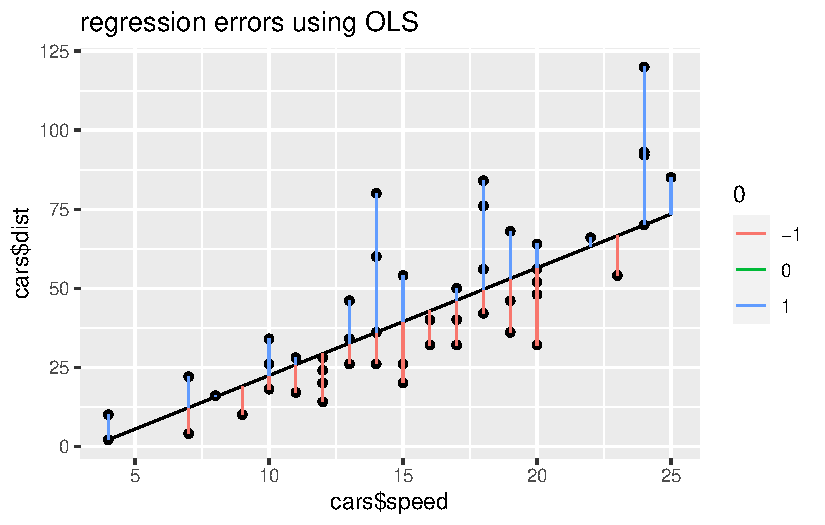
\includegraphics{methods_files/figure-pdf/unnamed-chunk-2-1.pdf}

}

\end{figure}

\begin{Shaded}
\begin{Highlighting}[]
\FunctionTok{table}\NormalTok{(color)}
\end{Highlighting}
\end{Shaded}

\begin{verbatim}
color
-1  0  1 
24  3 23 
\end{verbatim}

Notice that approximately half of the distribution of the points are
above the QR line and approximately half are above the QR line. Now
let's see what happens when we look at the 90th conditional quantile.

\begin{Shaded}
\begin{Highlighting}[]
\NormalTok{rq90 }\OtherTok{\textless{}{-}} \FunctionTok{rq}\NormalTok{(dist }\SpecialCharTok{\textasciitilde{}}\NormalTok{ speed, }\AttributeTok{data=}\NormalTok{cars, }\AttributeTok{tau=}\FloatTok{0.9}\NormalTok{)}
\NormalTok{yhat}\OtherTok{\textless{}{-}}\NormalTok{rq90}\SpecialCharTok{$}\NormalTok{fitted.values}
\NormalTok{color }\OtherTok{=} \FunctionTok{sign}\NormalTok{(rq90}\SpecialCharTok{$}\NormalTok{residuals)}
\FunctionTok{qplot}\NormalTok{(}\AttributeTok{x=}\NormalTok{cars}\SpecialCharTok{$}\NormalTok{speed, }\AttributeTok{y=}\NormalTok{cars}\SpecialCharTok{$}\NormalTok{dist)}\SpecialCharTok{+}\FunctionTok{geom\_line}\NormalTok{(}\AttributeTok{y=}\NormalTok{yhat)}\SpecialCharTok{+}
       \FunctionTok{geom\_segment}\NormalTok{(}\FunctionTok{aes}\NormalTok{(}\AttributeTok{x=}\NormalTok{cars}\SpecialCharTok{$}\NormalTok{speed, }\AttributeTok{xend=}\NormalTok{cars}\SpecialCharTok{$}\NormalTok{speed, }\AttributeTok{y=}\NormalTok{cars}\SpecialCharTok{$}\NormalTok{dist, }\AttributeTok{yend=}\NormalTok{yhat, }\AttributeTok{group=}\FunctionTok{as.factor}\NormalTok{(color), }\AttributeTok{color=}\FunctionTok{as.factor}\NormalTok{(color)))}\SpecialCharTok{+}
       \FunctionTok{labs}\NormalTok{(}\AttributeTok{title=}\StringTok{"regression errors"}\NormalTok{, }\AttributeTok{color=}\NormalTok{color)}
\end{Highlighting}
\end{Shaded}

\begin{figure}[H]

{\centering 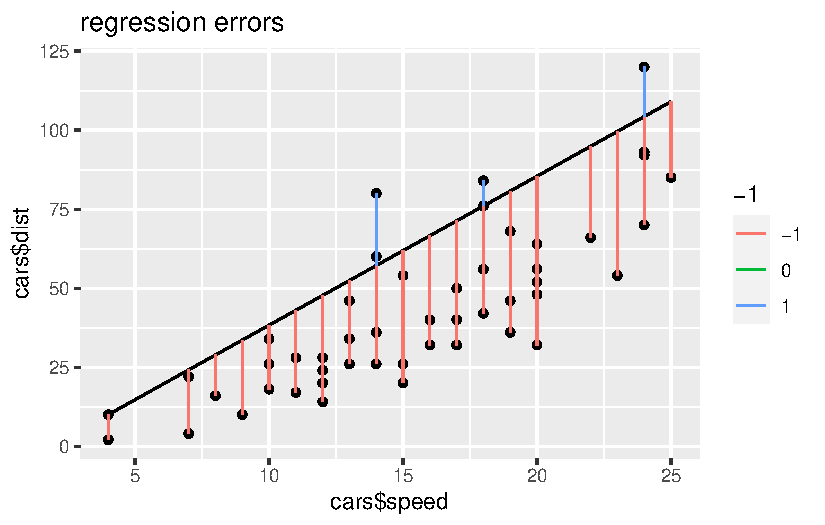
\includegraphics{methods_files/figure-pdf/unnamed-chunk-4-1.pdf}

}

\end{figure}

\begin{Shaded}
\begin{Highlighting}[]
\FunctionTok{table}\NormalTok{(color)}
\end{Highlighting}
\end{Shaded}

\begin{verbatim}
color
-1  0  1 
44  2  4 
\end{verbatim}

When we input the .9 for the quantile, we get approximately 90\% of the
points under the QR line and 10\% over the QR line.

\begin{Shaded}
\begin{Highlighting}[]
\NormalTok{rq10 }\OtherTok{\textless{}{-}} \FunctionTok{rq}\NormalTok{(dist }\SpecialCharTok{\textasciitilde{}}\NormalTok{ speed, }\AttributeTok{data=}\NormalTok{cars, }\AttributeTok{tau=}\FloatTok{0.1}\NormalTok{)}
\NormalTok{yhat}\OtherTok{\textless{}{-}}\NormalTok{rq10}\SpecialCharTok{$}\NormalTok{fitted.values}
\NormalTok{color }\OtherTok{=} \FunctionTok{sign}\NormalTok{(rq10}\SpecialCharTok{$}\NormalTok{residuals)}
\FunctionTok{qplot}\NormalTok{(}\AttributeTok{x=}\NormalTok{cars}\SpecialCharTok{$}\NormalTok{speed, }\AttributeTok{y=}\NormalTok{cars}\SpecialCharTok{$}\NormalTok{dist)}\SpecialCharTok{+}\FunctionTok{geom\_line}\NormalTok{(}\AttributeTok{y=}\NormalTok{yhat)}\SpecialCharTok{+}
       \FunctionTok{geom\_segment}\NormalTok{(}\FunctionTok{aes}\NormalTok{(}\AttributeTok{x=}\NormalTok{cars}\SpecialCharTok{$}\NormalTok{speed, }\AttributeTok{xend=}\NormalTok{cars}\SpecialCharTok{$}\NormalTok{speed, }\AttributeTok{y=}\NormalTok{cars}\SpecialCharTok{$}\NormalTok{dist, }\AttributeTok{yend=}\NormalTok{yhat, }\AttributeTok{group=}\FunctionTok{as.factor}\NormalTok{(color), }\AttributeTok{color=}\FunctionTok{as.factor}\NormalTok{(color)))}\SpecialCharTok{+}
       \FunctionTok{labs}\NormalTok{(}\AttributeTok{title=}\StringTok{"regression errors"}\NormalTok{, }\AttributeTok{color=}\NormalTok{color)}
\end{Highlighting}
\end{Shaded}

\begin{figure}[H]

{\centering 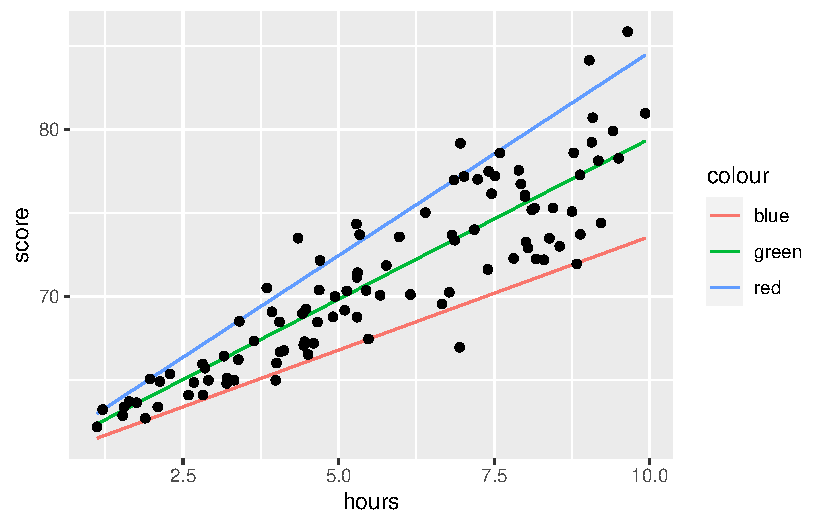
\includegraphics{methods_files/figure-pdf/unnamed-chunk-6-1.pdf}

}

\end{figure}

\begin{Shaded}
\begin{Highlighting}[]
\FunctionTok{table}\NormalTok{(color)}
\end{Highlighting}
\end{Shaded}

\begin{verbatim}
color
-1  0  1 
 5  1 44 
\end{verbatim}

When we input 0.1 for the 10th percentile, we get approximately 90\% of
the points above the QR line and 10\% below the QR line.

Thus, we can see that QR is not online a robust \#\# Evaluation metrics

\hypertarget{mean-absolute-error}{%
\subsection{Mean absolute error}\label{mean-absolute-error}}

The mean absolute error (MAE) is the average magnitude of the errors of
the values predicted by the regression and the actual observed values
for the response variable. Because it is a simple average, all errors
have the same weight, there are no penalties for different magnitude
deviations {[}2{]}. MAE assumes that the errors are normally
distributed, if the error distribution was non-normal, the average may
not be a good measure of centrality and can paint a false picture of the
goodness-of-fit of the regression curve. MAE also assumes that the
errors are unbiased. While the average magnitude of the errors is
expected to be non-zero (unless the regression is a perfect fit) the
average of the residuals, i.e., the deviation of the predicted value
from the actual value, considering underestimation and overestimation.
This means on average the regression curve does not over or
underestimate.

\[
\text { MAE }=\frac{1}{n}\sum_{i=1}^n\left|y_i-\hat{y}_i\right|=\frac{1}{n}\sum_{i=1}^n\left|e_i\right|
\]

\hypertarget{root-mean-squared-error}{%
\subsection{Root mean squared error}\label{root-mean-squared-error}}

It calculates the differences between the predictions and the actual
observations (residuals) and then gets their quadratic mean for each.
This type of error gives a larger penalty for larger errors {[}2{]}.
This error also assumes that the errors are unbiased and that they
follow a normal distribution. This gives a picture of the size of
residuals in comparison to the regression line.

\[
\operatorname{RMSE}=\sqrt{\operatorname{MSE}}=\sqrt{\frac{1}{n}\sum_{i=1}^n (y_i-\hat{y}_i)^2}=\sqrt{\frac{1}{n}\sum_{i=1}^n e_i^2}
\]

\hypertarget{variance-of-error}{%
\subsection{Variance of error}\label{variance-of-error}}

It is a measure of how spread all the errors are from the mean of all
errors.

\[
\operatorname{Var}(e)=\frac{1}{n}\sum_{i=1}^n(e_i-\bar{e})^2
\]

\hypertarget{minmax-error}{%
\subsection{Min/max error}\label{minmax-error}}

A measure of the maximum residual for a prediction and the minimum
residual.

\[
f: X \rightarrow \mathbb{R} \text {, if }(\forall e \in X_{error}) f\left(e_i\right) \geq f(e)
\]

\[
f: X \rightarrow \mathbb{R} \text {, if }(\forall e \in X_{error}) f\left(e_i\right) \leq f(e)
\]



\end{document}
